\subsection{SchedRR vs SchedRR2}

Para comparar el funcionamiento de los dos schedulers simularemos el comportamiento de ambos algoritmos utilizando tres lote de tareas:
\begin{itemize}
	\item Lote 1: combina varias tareas de uso intensivo de CPU y tareas interactivas (bloqueantes). La idea es simular un lote que podría estar corriendo en cualquier computadora hogareña. Este lote tendrá 180 tareas que es la cantidad de procesos corriendo actualmente en esta computadora.
	\item Lote 2: conformada por tareas de tipo interactivas. Simulará a un lote de tareas de un celular.
	\item Lote 3: conformada por tareas que solo hacen uso intensivo de CPU.
\end{itemize}
Para cada uno de los lotes calcularemos el waiting time y turnaround time promedio para cada scheduler tomando distintos valores de quantum y probando con 2, 3 y 4 cores. Teniendo en cuenta los resultados concluiremos cuál de los dos algoritmos se comporta mejor.

\begin{figure}
\hfill
\subfigure[]{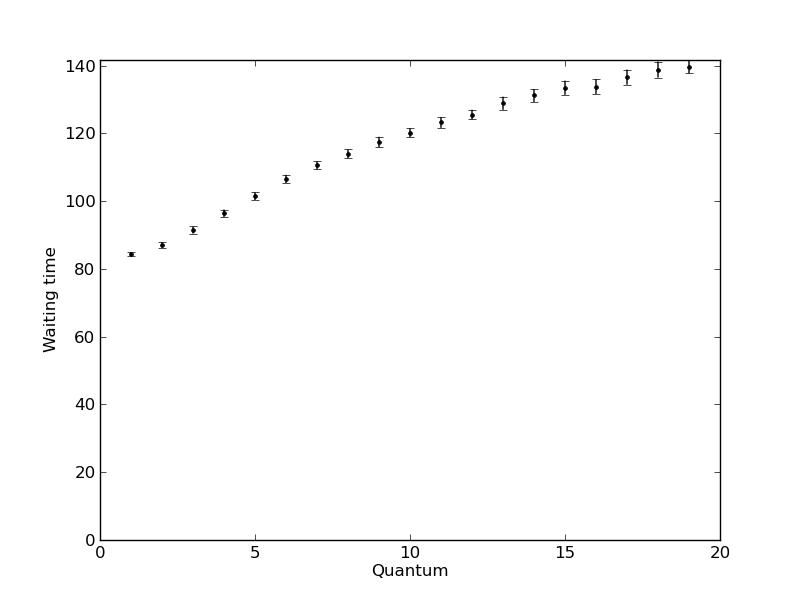
\includegraphics[width=8.75cm]{graficos/schedRR_pc/cores_2_wt.jpg}}
\hfill
\subfigure[]{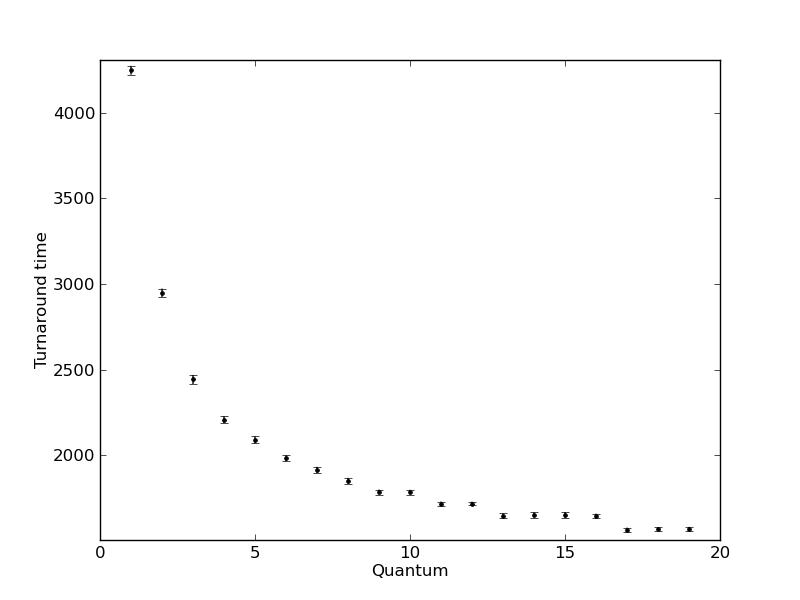
\includegraphics[width=8.75cm]{graficos/schedRR_pc/cores_2_ta.jpg}}
\hfill
\caption{Gráfico de Waiting time y turnaround time en función del quantum con 2 cores para lote de tareas $lotePc$}
\end{figure}

\begin{center}
    \begin{tabular}{ | l | l | l | p{5cm} |}
    \hline
    Cores & Waiting time promedio & Turnaround time \\ \hline
    2 & asd & asd \\ \hline
	3 & asd & asd \\ \hline
	4 & asd & asd \\
	\hline
    \end{tabular}
\end{center}
